

%\renewcommand{\Titulo}{A Platform for e-Health Control and Location Services for Wandering Patients~}

\begin{frame}{\citetitle{MarcoNuno_Revista_2018_03_00} \footnotemark (1)}
\begin{block}{Problem Description } 
%\begin{columns}
%\begin{column}{0.4\textwidth}
		\begin{itemize}
		\item Dementia refers to the loss of cognitive functioning.  
\note[item]{\scriptsize 	People suffering from dementia are affected in their ability to think, remember, and reason. The most common causes of dementia are Alzheimer’s disease, vascular dementia, among others}
		\item Wandering patients frequently have diseases that demand continuous health control.
%\note[item]{\scriptsize such as taking pills at specific times, constant blood pressure and heart rate monitoring, temperature and stress level checkups, and so on.}
		\item Sensor-based applications are highly energy demanding.
%\note[item]{\scriptsize they can be unaffordable in mobile e-health control due to battery constraints.}		
        \item We propose the design and implementation of a platform to provide support in e-health control and provision of location services for wandering patients
\note[item]{\scriptsize The proposed system perfroms real-time medical and mobility information analysis.}
		\end{itemize}
%\end{column}
%\begin{column}{0.6\textwidth}  
    
%\end{column}
%\end{columns}
\end{block} 
\footnotetext[1]{\fullcite{MarcoNuno_Revista_2018_03_00}}
\setcounter{footnote}{0}
\end{frame}


\begin{frame}{\citetitle{MarcoNuno_Revista_2018_03_00} (2)}
\begin{block}{Proposed solution}
\begin{columns}
\begin{column}{0.4\textwidth}
Main components:
\begin{itemize}
\item Mobile application
\item Smartband
\item Web service
\end{itemize}
Readings managed in the system:
\note[item]{\scriptsize The data packages transmitted to the Cloud service are integrated by the following sets of sensor-based information }
\begin{itemize}
\item TS (Time Stamp)
\item HR (Heart Rate)
\item GPS Locattion
\item SL (Stress Level)
\item PA (Physical Activity)
\end{itemize}
%\note[item]{\scriptsize The Mobile Application manages the information in three phases: In the first stage, a mobile app reads vital signs, GPS, and stress level making use of a smartband; In the second stage the medical and location information is transmitted to a Cloud-based storage system, which works as an interface between the mobile application and the web service; and in the third stage the information is appropriately managed and analyzed in the web service to assist the patient when abnormal medical states and location behavior are detected.}
\note[item]{\scriptsize The platform allows caregivers to manage personal information from wandering patients, including reviewing and following up biomedical readings. }

% The main functionality of the cloud storage is to secure the information of the wandering patients for further analysis. It enables storing large data sets for heart rate, stress, and location monitoring services, which can be accessed when required.

% The platform allows caregivers to manage personal information from wandering patients, including reviewing and following up biomedical readings



\end{column}
\begin{column}{0.6\textwidth}
    \begin{center}
         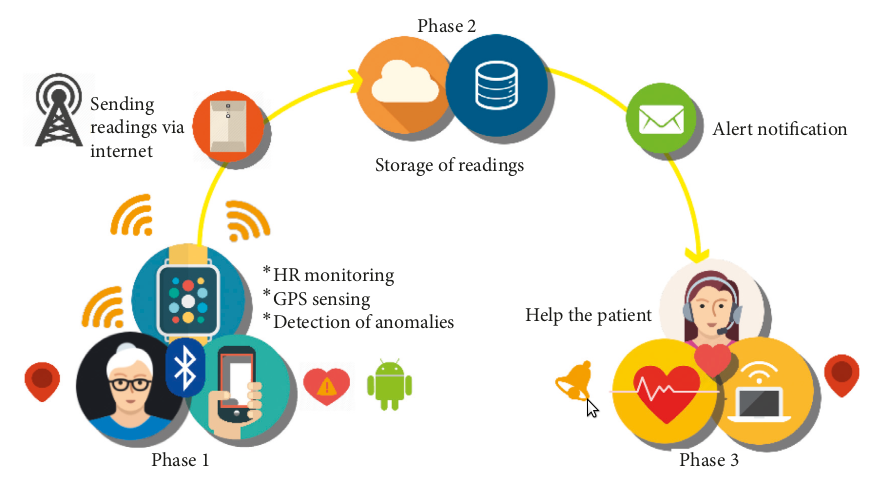
\includegraphics[width=0.96\textwidth]{Figs/SignosVitales1}
     \end{center}
\end{column}
\end{columns}
\end{block}


\end{frame} 


\begin{frame}{\citetitle{MarcoNuno_Revista_2018_03_00} (3)}
\begin{block}{Mobile App Screens}
\begin{columns}
\begin{column}{0.24\textwidth}
\begin{itemize}
\item Login
\item User and contact registration
\item Main Activity
\item Parameter settings
\item Energy saving settings
\end{itemize}
\end{column}
\begin{column}{0.39\textwidth}
    \begin{center}
         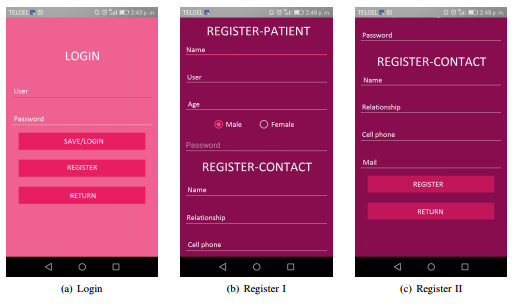
\includegraphics[width=1.0\textwidth]{Figs/Dementia_modulosA}
%         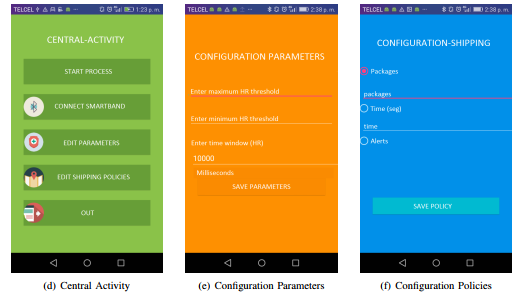
\includegraphics[width=1.0\textwidth]{Figs/Dementia_modulosB}
     \end{center}
     \end{column}
     \begin{column}{0.39\textwidth}
    \begin{center}
 %        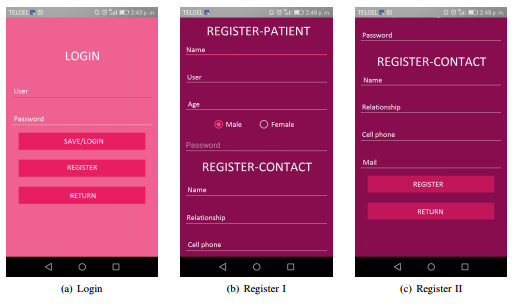
\includegraphics[width=1.0\textwidth]{Figs/Dementia_modulosA}
         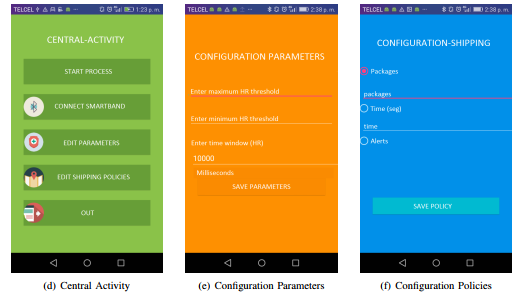
\includegraphics[width=1.0\textwidth]{Figs/Dementia_modulosB}
     \end{center}
     
          \end{column}
\end{columns}

\note[item]{\scriptsize The login is intended to authenticate users...}
\note[item]{\scriptsize User and contact registration screen allows to register the patient information and contact information. }
\note[item]{\scriptsize  The central activity shows a other functions. }
\note[item]{The first runs the service in the background of the HR monitoring, location sensing, and patient activity.}
\note[item]{Another function searchs and pairs the app with the external smartband. } 
\note[item]{A third option sets Heart Rate thresholds, as well as a time window value, for identifying abnormal readings.}
\note[item]{\scriptsize  Another option allow the configuration of energy-efficient handling and transmission policies}
\end{block}
\end{frame} 




